\documentclass[type=bachelor]{thuthesis}
% 选项:
%   type=[bachelor|master|doctor|postdoctor], % 必选
%   secret,                                   % 可选
%   pifootnote,                               % 可选(建议打开)
%   openany|openright,                        % 可选,基本不用
%   arial,                                    % 可选,基本不用
%   arialtoc,                                 % 可选,基本不用
%   arialtitle                                % 可选,基本不用

% 所有其它可能用到的包都统一放到这里了,可以根据自己的实际添加或者删除。
\usepackage{thuthesis}

% 定义所有的图片文件在 figures 子目录下
\graphicspath{{figures/}}

% 可以在这里修改配置文件中的定义。导言区可以使用中文。
% \def\myname{薛瑞尼}

\begin{document}

%%% 封面部分
\frontmatter
\thusetup{
  %******************************
  % 注意:
  %   1. 配置里面不要出现空行
  %   2. 不需要的配置信息可以删除
  %******************************
  %
  %=====
  % 秘级
  %=====
  secretlevel={秘密},
  secretyear={10},
  %
  %=========
  % 中文信息
  %=========
  ctitle={虚拟容器管理系统设计与实现},
  cdegree={工学学士},
  cdepartment={计算机科学与技术系},
  cmajor={计算机科学与技术},
  cauthor={陈天昱},
  csupervisor={姜进磊副教授},
  % 日期自动使用当前时间,若需指定按如下方式修改:
  % cdate={超新星纪元},
  %
  % 博士后专有部分
  cfirstdiscipline={计算机科学与技术},
  cseconddiscipline={系统结构},
  postdoctordate={2009年7月——2011年7月},
  id={编号}, % 可以留空: id={},
  udc={UDC}, % 可以留空
  catalognumber={分类号}, % 可以留空
  %
  %=========
  % 英文信息
  %=========
  etitle={The Design and Implementation of a Linux Container Management System},
  % 这块比较复杂,需要分情况讨论:
  % 1. 学术型硕士
  %    edegree:必须为Master of Arts或Master of Science(注意大小写)
  %             “哲学、文学、历史学、法学、教育学、艺术学门类,公共管理学科
  %              填写Master of Arts,其它填写Master of Science”
  %    emajor:“获得一级学科授权的学科填写一级学科名称,其它填写二级学科名称”
  % 2. 专业型硕士
  %    edegree:“填写专业学位英文名称全称”
  %    emajor:“工程硕士填写工程领域,其它专业学位不填写此项”
  % 3. 学术型博士
  %    edegree:Doctor of Philosophy(注意大小写)
  %    emajor:“获得一级学科授权的学科填写一级学科名称,其它填写二级学科名称”
  % 4. 专业型博士
  %    edegree:“填写专业学位英文名称全称”
  %    emajor:不填写此项
  edegree={Bachelor of Engineering},
  emajor={Computer Science and Technology},
  eauthor={CHEN Tianyu},
  esupervisor={Associate Professor JIANG Jinlei},
  % 日期自动生成,若需指定按如下方式修改:
  % edate={December, 2005}
  %
  % 关键词用“英文逗号”分割
  ckeywords={虚拟化, 虚拟容器, 分布式系统, 性能测试, 应用自动部署},
  ekeywords={Virtualization, Linux Container, Distributed Systems, Benchmark, Application Automatic Deployment}
}

% 定义中英文摘要和关键字
\begin{cabstract}
  论文的摘要是对论文研究内容和成果的高度概括。摘要应对论文所研究的问题及其研究目
  的进行描述,对研究方法和过程进行简单介绍,对研究成果和所得结论进行概括。摘要应
  具有独立性和自明性,其内容应包含与论文全文同等量的主要信息。使读者即使不阅读全
  文,通过摘要就能了解论文的总体内容和主要成果。

  论文摘要的书写应力求精确、简明。切忌写成对论文书写内容进行提要的形式,尤其要避
  免“第 1 章……;第 2 章……;……”这种或类似的陈述方式。

  本文介绍清华大学论文模板 \thuthesis{} 的使用方法。本模板符合学校的本科、硕士、
  博士论文格式要求。

  本文的创新点主要有:
  \begin{itemize}
    \item 用例子来解释模板的使用方法;
    \item 用废话来填充无关紧要的部分;
    \item 一边学习摸索一边编写新代码。
  \end{itemize}

  关键词是为了文献标引工作、用以表示全文主要内容信息的单词或术语。关键词不超过 5
  个,每个关键词中间用分号分隔。(模板作者注:关键词分隔符不用考虑,模板会自动处
  理。英文关键词同理。)
\end{cabstract}

% 如果习惯关键字跟在摘要文字后面,可以用直接命令来设置,如下:
% \ckeywords{\TeX, \LaTeX, CJK, 模板, 论文}

\begin{eabstract}
   An abstract of a dissertation is a summary and extraction of research work
   and contributions. Included in an abstract should be description of research
   topic and research objective, brief introduction to methodology and research
   process, and summarization of conclusion and contributions of the
   research. An abstract should be characterized by independence and clarity and
   carry identical information with the dissertation. It should be such that the
   general idea and major contributions of the dissertation are conveyed without
   reading the dissertation.

   An abstract should be concise and to the point. It is a misunderstanding to
   make an abstract an outline of the dissertation and words ``the first
   chapter'', ``the second chapter'' and the like should be avoided in the
   abstract.

   Key words are terms used in a dissertation for indexing, reflecting core
   information of the dissertation. An abstract may contain a maximum of 5 key
   words, with semi-colons used in between to separate one another.
\end{eabstract}

% \ekeywords{\TeX, \LaTeX, CJK, template, thesis}

% 如果使用授权说明扫描页,将可选参数中指定为扫描得到的 PDF 文件名,例如:
% \makecover[scan-auth.pdf]
\makecover

%% 目录
\tableofcontents

%% 符号对照表
\begin{denotation}[3cm]
\item[LXC] 虚拟容器 (Linux Container)
\item[time-sharing] 分时
\item[AWS] 亚马逊云计算服务 (Amazon Web Services)
\item[IaaS] 基础设施服务 (Infrastructure as a Service)
\item[PaaS] 平台服务 (Platform as a Service)
\item[SaaS] 软件服务 (Software as a Service)
\item[hypervisor] 虚拟机管理程序
\item[instance] 虚拟机实例
\item[LAN] 局域网 (Local Area Network)
\item[VLAN] 虚拟局域网 (Virtual Local Area Network)
\item[SAN] 存储区域网络 (Storage Area Network)
\item[NAS] 网络附属存储 (Network Attached Storage)
\item[Object Storage] 对象存储
\item[Block Storage] 块存储
\end{denotation}



%%% 正文部分
\mainmatter
\chapter{引言}
\label{cha:intro}

\section{选题背景}

\subsection{云计算的历程}

云计算的概念诞生的远远比它的名字更早。它的概念可以追溯到早期的
分时系统\footnote{time-sharing systems}。

早期的计算机系统价格昂贵,而且体积庞大,使得个人用户很难拥有独立的个人计算机 (PC) 。
这就导致了多个用户可以同时使用同一个计算资源——例如一台电子计算机——的分时系统
~\cite{timesharing}的产生。所谓分时系统,就是有一个主要的
计算系统 (mainframe computer) ,用户通过终端机 (terminal) 连接到这个
系统上使用计算资源。用户一般而言不需要考虑计算机操作系统乃至硬件的具体细节——因为自然
有管理员管理这些细节,只需要像“租客”一样使用计算资源就可以了。现代的操作系统,
例如 GNU/Linux 或者 Microsoft Windows ,都支持多用户模式。

\begin{figure}[h]
    \centering
    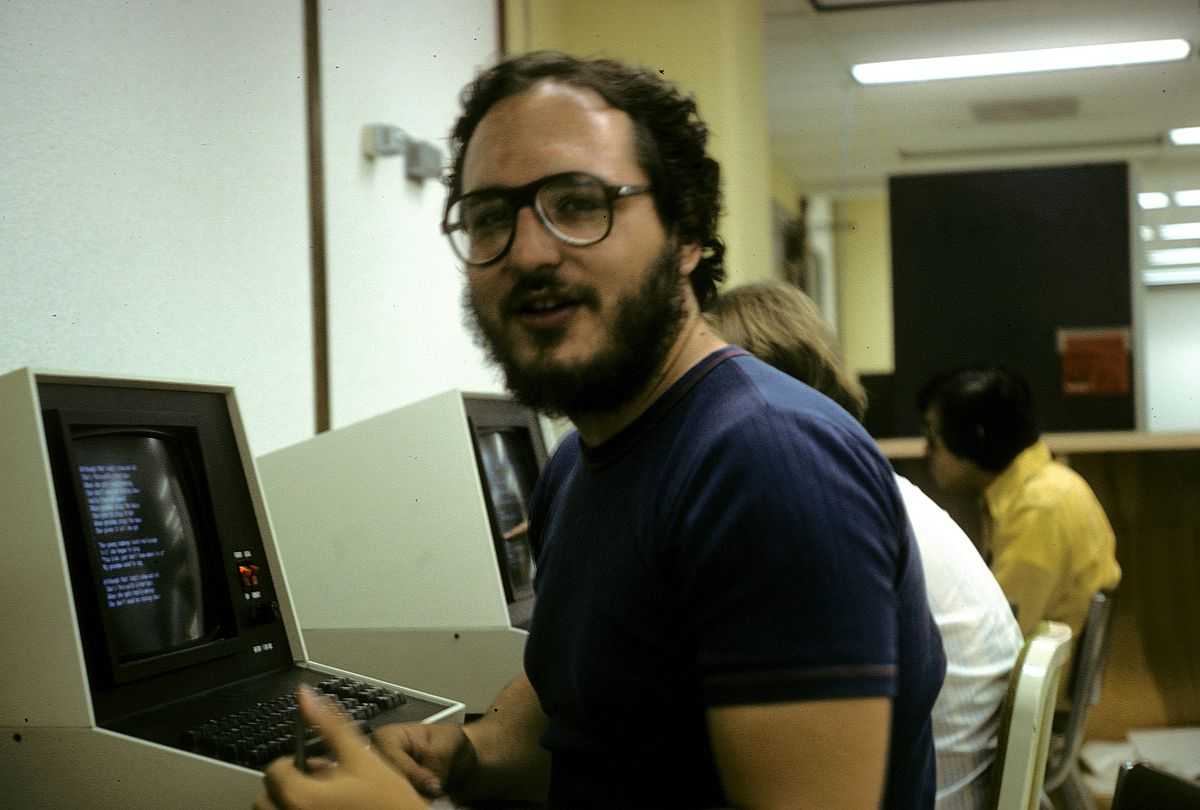
\includegraphics[height=0.5\textwidth]{unix_time_sharing}
    \caption{威斯康辛大学麦迪逊分校的学生使用终端机,1978 年}
\end{figure}

从 2000 年左右开始,云计算的概念正式形成了。2006 年诞生的 Amazon EC2 \footnote{EC2
  是 Elastic Compute Cloud 的缩写,因有两个连着的 C 所以叫做 EC2 ,不是
  “第二个版本”的意思。}成为了迄今最成功的云计算平台之一。2008 年诞生的 OpenNebula
是另一个云计算平台,顾名思义它是一个自由软件\footnote{Free as in freedom}
,使用 Apache License 发布。

而现在更加流行的自由的云计算平台是 OpenStack 。OpenStack 最初是由
 NASA 和 RackSpace 共同发起的,从 2012 年开始由叫做 OpenStack Foundation 的非营利
组织进行开发和维护。它和 Amazon EC2 的最大不同就是它是完全自由和开源的。不但可以利用
这个软件搭建自己的云计算环境,而且可以对相关的代码展开研究。OpenStack 中的主要组成部分
和 Amazon AWS 中的部分具有一定的对应关系,比如 AWS 的核心也就是 EC2 对应了 OpenStack
 里的 Nova ,负责虚拟机的调度和管理;AWS 中的简单存储模块 S3 在 OpenStack 中
有 Swift 与之对应~\cite{openstack}。

\subsection{云计算平台的服务类型}

云计算提倡的概念是“所有都是服务”
 (everything as a service) ~\cite{cloud-and-openstack},也就是用户不直接接触
物理上的计算机,但是却能通过网络获得相应的计算服务。云计算的“云”不在本地,这就好比大家
每天日常生活都要使用电,但极少有人在家里自己搭建一台柴油发电机,而是在发电厂集中发电,
然后通过输电线路把电力输送到千家万户供人们使用。数据中心就好像这个发电厂,计算机网络
就好像电线,终端用户就像使用电力一样使用云计算产生的计算资源。

根据服务类型不同,云计算平台主要可以分为以下三种——基础设施
服务 (IaaS)、平台服务 (PaaS) 还有软件服务 (SaaS) ~\cite{types-of-cloud}。

\subsubsection{基础设施服务}

顾名思义,这种服务类型就是只提供必要的设施,而不提供上层应用。这些设施包括由虚拟机管理程序
支持的大量的虚拟机集群、操作系统磁盘镜像存储池(这样用户在创建虚拟机实例的时候就不用联网
从镜像源下载镜像,直接从镜像存储服务调取相应的镜像即可)、文件存储服务、防火墙、负载均衡器
等等。

当然还有虚拟局域网。例如某大学计算机系有网络和操作系统两个实验室,它们共享一套虚拟机集群。
网络实验室和操作系统实验室希望各占用一个子网。如果是使用物理上的局域网,那么应该有两个交换机,
各接入路由器的两个物理端口上。而使用了虚拟局域网,就可以用两个逻辑端口代替。使用虚拟局域网,
可以缩小广播域,从而提高集群的安全性。

上文提到的 Amazon EC2 就是一个典型的 IaaS 平台。类似的,OpenStack 也是一个 IaaS 平台,
截至到 2016 年,一共包含以下几个核心组成部分~\cite{openstack}:

\begin{enumerate}
    \item \textbf{Nova:} Nova 是 OpenStack 的计算部分,主要负责虚拟机管理。它的 API
    可以和 Amazon EC2 的相兼容,RackSpace 的商业计算服务就是建立在 Nova 上的。
    \begin{enumerate}
        \item \textbf{nova-compute}
        \item \textbf{nova-scheduler}
        \item \textbf{nova-conductor}
        \item \textbf{nova-db}
        \item \textbf{nova-console}
        \item \textbf{nova-cert}
        \item \textbf{nova-objectstore}
    \end{enumerate}
    \item \textbf{Neutron:}
    \item \textbf{Swift:}
    \item \textbf{Cinder:}
    \item \textbf{Keystone:}
    \item \textbf{Glance:}
\end{enumerate}


\subsubsection{平台服务}

\subsubsection{软件服务}

\subsection{虚拟化和云计算}

\section{研究价值和主要贡献}

\section{论文结构}



%%% 其它部分
\backmatter

%% 本科生要这几个索引,研究生不要。选择性留下。
% 插图索引
\listoffigures
% 表格索引
\listoftables
% 公式索引
\listofequations


%% 参考文献
% 注意:至少需要引用一篇参考文献,否则下面两行可能引起编译错误。
% 如果不需要参考文献,请将下面两行删除或注释掉。
\bibliographystyle{thuthesis}
\bibliography{ref/refs}


%% 致谢
% 如果使用声明扫描页,将可选参数指定为扫描后的 PDF 文件名,例如:
% \begin{ack}[scan-statement.pdf]
\begin{acknowledgement}
待完成
\end{acknowledgement}


%% 附录
\begin{appendix}
	\chapter{外文资料的调研阅读报告或书面翻译}

\title{Xen 与虚拟化的艺术}

{\heiti 摘要:} 人们设计了无数的系统以通过虚拟化技术分享现代计算机的充足的计算资源。
其中,有的系统需要特制的硬件,或者不能运行日常使用的操作系统;有的为了百分之百的二进制兼容
不得不以性能作为代价;还有的为了性能好牺牲了安全性和功能性。只有很少的一部分提供资源隔离和
性能的保障,大多数只提供“尽力而为”的表现,承担着很高的拒绝服务风险。

在本文中,一个叫做 Xen 的 X86 虚拟化管理程序被提出出来。它使多个常见的操作系统可以以安全、
资源可控而且性能功能都有保障的方式,共享传统的硬件设备。这是通过提供理想化的虚拟机抽象达到的,
常见的操作系统例如 Linux 、 BSD 还有 Windows XP 可以只需很少的努力移植到这个平台。

我们的设计指标允许多达 100 台虚拟机实例在一台物理服务器主机上同时运行。我们采用的虚拟化方法
是非常高效的,例如 Linux 和 Windows XP 的操作系统可以在我们的平台上以极少的性能开销共同
运行——相较于直接运行在物理机上只有百分之个位数的开销。无论在微基准测试,还是在全系统的测试上,
我们的系统都极大地超越了与其竞争的商业和免费的现有解决方案。

\section{引言}

现代的计算机足够强大,可以通过虚拟化技术启动许多小的“虚拟机”,并在每个虚拟机上运行一个独立的
操作系统实例。这导致了虚拟化技术研究兴趣的回潮。在本文中,我们提出了 Xen ,一个高性能、资源
可控的虚拟机管理程序,它可以支持服务器联合、协同托管服务、分布式 web 服务、安全计算平台和
应用程序移动性等多种应用。

成功地将一台主机划分成并行执行的多个操作系统具有以下几个挑战:首先,虚拟机必须保证互相隔离,
它们的执行过程互相影响是不能接受的。尤其是在虚拟机被多个互相不信任的用户共同使用的情况下。
其次,必须支持多种操作系统,才能适应流行的应用程序的多样性。最后,虚拟化带来的开销应该尽可能小。

Xen 可以承载常见的操作系统,尽管需要进行源代码的更改。本文中描述和评估的 Xen 样本支持多个
并行执行的 XenoLinux 客户操作系统实例,每个实例向上对应用程序提供和非虚拟化的 Linux 2.4
完全相同的二进制接口。我们对 Windows XP 的移植虽然是不完整的,但是已经可以运行简单的用户态
应用程序。我们还在移植 NetBSD 操作系统。

Xen 允许用户动态地实例化一个操作系统,使其可以在用户希望的任何地方运行。在 XenoLinux
项目中,我们在互联网提供商和互联网交换机的较为经济的位置上的物理节点上部署了 Xen 系统。
我们在它开启新的虚拟机前进行了准入控制,并且希望每个虚拟机为它所需的资源付出相应的“代价”。
我们会在另外的地方从这个角度讨论我们的想法和实现方法,本文更多地还是关注虚拟机管理程序本身。

在一个共享的物理系统上部署多种应用程序和服务有很多种方法,其中很可能是最简单的一种就是部署
多个主机,每个运行一个标准的如 Linux 或者 Windows 的操作系统,然后用户可以安装文件、
开启程序,应用程序之间的保护机制是由传统的操作系统技术实现的。经验表明,如果这样做,系统
管理工作很快就会变成一项耗时的任务,因为本该互相隔离的应用程序之间复杂的交互配置。

更重要的是,这种系统支持的性能隔离还不够——一个进程的调度优先顺序、内存需求、网络流量还有
磁盘访问会直接影响其它程序的。对于事先规划好的固定的用户群体,这个也许是可以接受的(比如
网格计算或者实验性的 PlanetLab 平台),但是如果资源被过度订阅,或者用户互相协作不愉快,
那么这个模式就不可行。

一个解决方式是翻新操作系统本身对于性能隔离的支持。Resource container 技术、Linux/RK 、
QLinux 和 SILK 或多或少都表现出这个思想。一个主要的困难是保证所有资源占用的帐都记到正确的
那个进程的头上——尤其是考虑到例如缓冲区缓存或者页置换算法导致的应用程序之间复杂的交互。在
操作系统内部这是被称为“QoS crosstalk“的问题。降低复用率可以缓解这个问题,正如 Exokernel
和 Nemesis 操作系统展示的那样。在它们的实现中非刻意的或者不需要的进程间交互被降低到了最低。

我们使用类似的基本方法来创造 Xen ,在 Xen 中物理资源被以整个操作系统的粒度进行复用,
并且能提供它们之间的性能隔离。和进程级的复用不同的是,这种复用允许多个不同的客户操作系统
优雅地共同存在,而不是使用同一个应用层二进制接口。当然,这样的灵活性肯定要付出代价——运行整个
完整的操作系统肯定比运行单个进程更加“重量”,无论是从开机启动来说,还是从资源消耗来讲。

对于我们的目标也就是多达 100 个承载的虚拟机实例,我们相信上述代价是值得的,因为它单个用户
以资源可控制的方式运行未经修改的二进制或者一族二进制程序,例如一个 Apache 服务再加上一个
PostgreSQL 后端)。另外,它还提供了极致的灵活性,因为用户可以精确地恰到好处地创建那个
应用需要的运行环境。麻烦的在多个服务和应用之间的配置协调被避免了(比如说,每个 Windows 实例
可以维护自己独立的注册表)。

本论文的如下部分这样组织:在第二章我们介绍实现虚拟化的具体方法和 Xen 的基本工作原理。
在第三章介绍我们的设计和实现的一些关键细节。在第四章我们使用工业界标准的基准测试程序对在
Xen 上运行的 XenoLinux 内核与在物理机上运行的 Linux 内核、VMWare Workstation 还有
用户态 Linux (UML) 进行比较测试。第五章评价相关工作。第六章介绍后续工作和结论。

\section{Xen: 方法与概述}

在传统的虚拟机管理程序里,虚拟化软件对上层暴露出和下层的硬件完全相同的功能。尽管全虚拟化
有着显而易见的优点,也就是允许未经修改的操作系统在上面运行,但是它有几个缺点。对于流行的
IA-32 / X86 架构来说,更是如此。

对于全虚拟化的支持从来就不是 X86 体系结构的一部分。特定的内核指令必须经过虚拟机管理程序的
处理才能实现正确的虚拟化,但是在不足的权限下运行这些指令会悄无声息地失败,而不是导致易于
处理的陷入。高效率地将 X86 的 MMU 进行虚拟化也是非常困难的。这些问题当然都可以被解决,
只不过需要以增加的复杂度和降低的效率作为代价。VMWare 的 ESX Server 自动地重写一部分客户机
的代码来插入陷入,每当虚拟机管理程序必须介入执行的时候。这个翻译过程必须应用到整个客户机的
操作系统内核上(带来相应的翻译、执行、缓存的开销)因为所有不会带来陷入的特权指令必须被
捕获和处理。ESX Server 还实现了系统数据结构比如页表的一个“影子”版本,并且通过陷入每个
更新操作维护虚拟页表的一致性——这个实现方法对于更新频繁的操作,比如创建一个新的应用程序进程
带来了非常大的开销。

难以忍受 X86 错综复杂的特性,存在其它反对全虚拟化的讨论。特别是有客户虚拟机想要既能看到真实
的硬件资源又能看到虚拟的硬件资源的实际的应用情况,例如既提供实际的时钟又提供虚拟的时钟可以使
客户虚拟机更好地支持时间敏感的任务,使其准确地处理 TCP 超时以及 RTT 估计,又比如暴露出
物理机的实际地址允许客户机通过使用 superpages 和 page coloring 技术获得更好的性能表现。

我们通过提供一个和下层的硬件类似但是又不完全相同的虚拟机抽象来避免全虚拟化的缺陷——这种方法
被称为“半虚拟化”。这种方法会带来更高的性能,尽管需要修改客户机的操作系统。但是请注意,
我们不需要修改应用程序的二进制接口 ABI ,所以上层应用无须做修改。

我们将上述讨论总结为如下几个原则:

\begin{enumerate}
    \item 支持未经修改的应用程序二进制文件至关重要,否则用户就不会迁移到 Xen 。
    因此我们必须将现有的 ABI 的全部结构特性进行虚拟化;
    \item 支持完整的多任务操作系统是重要的,因为这样可以允许复杂的服务设置在单一的客户机
    操作系统实例内被虚拟化;
    \item 在 X86 这种虚拟化不友好的平台上,半虚拟化是必须的,因为通过它可以获得高性能
    和强的资源隔离;
    \item 即便在虚拟化友好的硬件架构上,完全地对客户操作系统隐藏虚拟化的效用也会带来正确性
    与性能的风险。
\end{enumerate}

注意,我们的 X86 半虚拟化抽象和最近的 Denali 项目提出的设计非常不同。Denali 被设计用来
支持数以千计的运行网络服务的虚拟机,它们中大多数都规模不大并且也不流行。形成对比的是,Xen
的设计目标是支持多达 100 个运行行业标准的应用与服务的虚拟机。因为目标非常不同,将 Denali
的设计方法和我们的原理作对比是有益的。

首先,Denali 的目标不在于已有的 ABI ,所以可以从虚拟机接口中忽略一部分结构特性。
举例来说,Denali 并不完全支持 X86 的分段机制,尽管它在 NetBSD 、Linux 和 Windows XP
的 ABI 中广泛使用。

其次,Denali 的实现方法没有解决支持应用程序复用或者一个客户操作系统的不同的地址空间的问题。
应用程序被以类似 Exokernel 中的 libOS 的形式显式地链接向一个 Ilwaco 客户操作系统的实例。
因此,每个虚拟机只能承载一个单用户模式的单应用的未经保护的所谓“操作系统”。形成对比的是,
在 Xen 中,一个虚拟机可以承载一个真正的操作系统,在这个操作系统上又可以复用出成千上万的
未经修改的用户态进程。尽管一个原型虚拟 MMU 被开发出来用于帮助 Denali 达到类似的目标,
但是我们没有看到任何已发表的技术细节或者评估报告。

再次,在 Denali 的架构中虚拟机管理程序通过磁盘输入输出操作所有分页机制。这可能是因为在
虚拟化层缺少内存管理机制。在虚拟机管理程序内部解决分页机制和我们的进行性能隔离的目标向左:
恶意的虚拟机会激励内存抖动,不公平地把别的虚拟机的 CPU 时间和磁盘带宽据为己有。在 Xen 系统中
我们希望每个客户机都有自己的分页机制,使用自己分配到的那一份内存空间和磁盘份额。

最后,Denali 将每台机器的资源的命名空间进行了虚拟化,采用了如果一台虚拟机不能对另一台虚拟机
的资源进行命名那么就无法访问该资源的方式。举例来说,虚拟机们对硬件地址一无所知,它们只知道
Denali 为它们创建的虚拟地址。相反,我们认为虚拟机管理程序内部的安全访问管理对于保护来说
已经足够了,另外,正如上文讨论过的,如果使物理资源被客户操作系统直接访问会带来很激烈的正确性
与性能的争论。

在下面的一节中我们讨论 Xen 的虚拟机抽象,并讨论 Xen 如何通过修改客户操作系统来达到这一点的。
注意,在本文中,我们使用术语“客户操作系统”来指代 Xen 可以承载的操作系统之一,使用“域”来指代
一个运行着某个“客户操作系统”的虚拟机;这个区别好似在传统的系统中程序与进程的概念。我们管 Xen
本身叫做虚拟机管理程序 (hypervisor) 因为它执行的特权级相对于它承载的客户操作系统的内核更高。

\subsection{虚拟机接口}

表 1 展示了 X86 半虚拟化接口的一个概览,主要可以划分为三个大块:内存管理、CPU 还有
输入输出设备。在下面的章节我们依次介绍三个子系统,并讨论每个部分是如何在我们的半虚拟化架构中
被表示的。注意,尽管我们的实现中的一部分,比如内存管理,是特定地针对 X86 平台的,许多方面
例如虚拟 CPU 和输入输出设备可以直接应用到别的体系结构上。另外,X86 体系结构代表了它区别于
RISC 体系结构的最坏的一种可能性,比如说,有效地将硬件页表虚拟化比将软件控制的 TLB
虚拟化要更加复杂。

\subsubsection{内存管理}

将内存虚拟化毫无疑问是将体系结构半虚拟化中最困难的部分,无论是从虚拟机管理程序的原理上讲,
还是从每种客户操作系统被移植的工作量上讲。如果体系结构本身提供一个软件管理的 TLB 那么这个
工作就更加容易了,因为这样的结构能简单有效地被虚拟化。TLB 标记是另一种被多数服务器级的 RISC
体系结构支持的有用的功能,比方说 Alpha 、MIPS 还有 SPARC 。将地址空间标志位同每个 TLB
表项联系起来使得虚拟机管理程序与每个客户操作系统有效地在分开的地址空间里共同存在,因为在二者
转换执行的时候就没有必要清空掉整个 TLB 了。

遗憾的是,X86 并没有软件控制的 TLB ,与此相反的是 TLB 缺失被 CPU 本身以遍历整个页表结构
的形式自动处理。因此为了达到最好的性能,所有有效的对于当前的地址空间内的页地址转换都需要在硬件
可访问的页表中存在。另外,因为 TLB 没有标记,地址空间转换通常需要清空整个 TLB 。基于这些限制,
我们作出了两个决定:(1) 客户操作系统负责分配和管理硬件页表,Xen 的介入非常至少来保证安全性
和隔离性;(2) Xen 在每段地址空间的上 64 MB 存在,因此避免进入退出虚拟机管理程序造成的 TLB
清空。

每次一个客户操作系统需要一个新的页表——也许是因为一个新的进程创建了——它从它自己的内存保留
区域内分配并初始化一页并在 Xen 上做登记。此时,操作系统必须放弃对页表所在的内存区域直接写入
的权限,之后所有的更新都需要被 Xen 批准。更新在几个方面被限制,包括只允许操作系统对它拥有的页
进行映射,并且禁用页表的可写入映射。客户操作系统可以通过一次送入一批更新请求的方式来减少进入
虚拟机管理程序的开销。每个地址空间上方 64MB 预留给 Xen ,对于客户操作系统是不可访问或者
重新映射的。这个地址区域不被任何常见的 X86 ABI 使用,所以这个限制不会影响应用程序的兼容性。

分段被用类似的方式进行虚拟化,就是批准对硬件段描述符表的更新。X86 里的段描述符惟独的限制是:
(1) 它们的特权级比 Xen 低;(2) 它们不允许任何对 Xen 预留的地址空间的访问。

\subsubsection{CPU}

对 CPU 进行虚拟化对于客户操作系统来说有几个含义:首先,在客户操作系统下方插入虚拟机管理程序
和传统意义上的“操作系统才是特权最高的”的概念相违背。为了保护虚拟机管理程序免于操作系统的
异常行为(以及域与域之间的隔离),客户操作系统必须进行修改在更低的特权级上运行。

很多的处理器体系结构只提供两个特权级。在这种情况下,客户操作系统会与应用程序一起共享较低的
特权级。客户操作系统通过在与应用程序不同的地址空间里运行而把自己保护起来,通过虚拟机管理程序
设置虚拟的特权级和改换当前地址空间从而间接地与应用程序交替运行。如果处理器的 TLB 支持地址空间
标记,那么代价昂贵的 TLB 清空就可以被避免了。

高效地将特权级进行虚拟化在 X86 上是可行的,因为它在硬件层面支持四个不同的特权级。X86 的特权级
一般被称为 rings ,从 0 到 3 。操作系统的代码通常在 ring 0 执行,因为其它的 ring 都不能
执行特权指令,而 ring 3 一般被应用程序的代码使用。据我们所知,ring 1 和 ring 2 自从 OS/2
就没有被任何著名的 X86 操作系统使用过。任何符合这个特点的操作系统都可以被移植到 Xen 上通过
修改以在 ring 1 里运行。这可以防止客户操作系统直接运行特权指令,并且可以和 ring 3 上运行的
应用程序隔离开来。

特权指令通过在 Xen 内部批准和执行来半虚拟化。这些适用于类似创建一个新的页表或者在空闲时放弃
CPU 资源等操作。任何客户操作系统的直接执行特权指令的尝试都会被处理器本身拒绝掉,或者是静默地
或者产生一个错误,因为只有 Xen 本身才能在一个权限足够的层级运行。

异常,包括内存异常和软件的陷入,在 X86 上的虚拟化都十分直接。描述每种异常的处理程序的表在
Xen 上登记待批准。这些在表中声明的处理程序基本上和对于真实 X86 硬件的相同。这是可行的,
因为在我们的半虚拟化架构中异常的栈帧没有被修改。唯一的修改是对于缺页异常的处理程序,它通常是
从特权寄存器 CR2 中读取缺页的地址,但是因为这是不可能的,我们把它写在了一个扩展的栈帧里。
每当一个异常发生在在 ring 0 外执行,Xen 的处理程序创建客户操作系统上异常栈帧的一个拷贝,
然后把控制权交给注册的处理程序。

通常,只有两类异常的发生会频繁到影响系统性能的地步:系统调用(它们通常是通过软件异常实现的)
还有缺页异常。我们通过允许每个客户机操作系统注册一个“快的”异常处理程序,它可以被处理器直接访问
而不是间接通过 ring 0,来提高系统调用的性能。这个处理程序在被写到硬件异常表中之前就被有效化了。
遗憾的是,不能对缺页处理程序使用相同的技术,因为只有 ring 0 里执行的代码才能访问 CR2 里
存储的缺页地址,缺页异常必须通过 Xen 被传送一次,使得寄存器的值能从 ring 1 中访问。

安全性是由直到异常处理程序被传给 Xen 才被有效化而保证的。唯一需要的检查是处理程序的代码段
不会提出去 ring 0 执行。因为没有客户操作系统能创建类似的段,它有能力比较那个段选择子与 Xen
预留的几个静态的值之间的大小关系。除此之外,其它的一些处理程序的问题会在异常的传输过程中被解决
——举例来说,如果处理程序的代码段不存在或是处理程序没有被进行内存分页,那么当 Xen 执行 iret
指令返回处理程序的时候,相应的异常就会被处理。Xen 通过检查异常程序的计数器来检测“双误”
(double faults) ,如果地址处于异常虚拟化的代码处,那么触犯的客户操作系统会被终止。

请注意,即使对于直接的系统调用处理程序,惰性检查也是安全的,因为访问异常只有当 CPU 尝试直接
跳转到客户操作系统的处理程序时才会发生。在这种情况下,异常的地址是在 Xen 之外的,因为 Xen
永远也不会调用客户操作系统的系统调用,所以异常被虚拟化的方法是正常的。如果异常在传导过程中
导致了双误,那么客户操作系统会被以如上方式终止。

\subsubsection{设备 I/O}

和全虚拟化环境中模拟现实存在的硬件设备不同的是,Xen 暴露出的是清晰而简单的设备抽象。
这就允许我们设计出一个既高效又满足对于保护和隔离的需要的接口。为此,I/O 数据通过 Xen
在各个域之间传递,使用的是共享内存的、异步的缓冲区描述符的环 (buffer-descriptor rings) 。
这就提供了一个高效的在系统中垂直传递缓冲区信息的通讯机制,Xen 可以借此实现高效率的有效性检查,
比如检查包含在域的保留内存内的缓冲区)。

与硬件中断相似,Xen 支持一种轻量的传送机制,它被用来向一个域发送异步的通知。这些通知是通过
更新待完成的事件类型的一个位映射实现的,也可以选择使用调用由客户操作系统指明的事件处理程序。
这些事件的回调可能会因为客户操作系统的决策而被暂缓——比如说为了减少因为频繁的唤醒导致的额外的开销。

\subsection{向 Xen 移植操作系统的开销}

表 2 通过代码行数展示了向 Xen 的半虚拟化环境移植常见操作系统的代价。注意我们的 NetBSD
移植尚处在非常初始的阶段,所以没把它的数据加入表格。

\end{appendix}

%% 个人简历
\begin{resume}

  \resumeitem{个人简历}

  xxxx 年 xx 月 xx 日出生于 xx 省 xx 县。

  xxxx 年 9 月考入 xx 大学 xx 系 xx 专业,xxxx 年 7 月本科毕业并获得 xx 学士学位。

  xxxx 年 9 月免试进入 xx 大学 xx 系攻读 xx 学位至今。

  \researchitem{发表的学术论文} % 发表的和录用的合在一起

  % 1. 已经刊载的学术论文(本人是第一作者,或者导师为第一作者本人是第二作者)
  \begin{publications}
    \item Yang Y, Ren T L, Zhang L T, et al. Miniature microphone with silicon-
      based ferroelectric thin films. Integrated Ferroelectrics, 2003,
      52:229-235. (SCI 收录, 检索号:758FZ.)
    \item 杨轶, 张宁欣, 任天令, 等. 硅基铁电微声学器件中薄膜残余应力的研究. 中国机
      械工程, 2005, 16(14):1289-1291. (EI 收录, 检索号:0534931 2907.)
    \item 杨轶, 张宁欣, 任天令, 等. 集成铁电器件中的关键工艺研究. 仪器仪表学报,
      2003, 24(S4):192-193. (EI 源刊.)
  \end{publications}

  % 2. 尚未刊载,但已经接到正式录用函的学术论文(本人为第一作者,或者
  %    导师为第一作者本人是第二作者)。
  \begin{publications}[before=\publicationskip,after=\publicationskip]
    \item Yang Y, Ren T L, Zhu Y P, et al. PMUTs for handwriting recognition. In
      press. (已被 Integrated Ferroelectrics 录用. SCI 源刊.)
  \end{publications}

  % 3. 其他学术论文。可列出除上述两种情况以外的其他学术论文,但必须是
  %    已经刊载或者收到正式录用函的论文。
  \begin{publications}
    \item Wu X M, Yang Y, Cai J, et al. Measurements of ferroelectric MEMS
      microphones. Integrated Ferroelectrics, 2005, 69:417-429. (SCI 收录, 检索号
      :896KM)
    \item 贾泽, 杨轶, 陈兢, 等. 用于压电和电容微麦克风的体硅腐蚀相关研究. 压电与声
      光, 2006, 28(1):117-119. (EI 收录, 检索号:06129773469)
    \item 伍晓明, 杨轶, 张宁欣, 等. 基于MEMS技术的集成铁电硅微麦克风. 中国集成电路,
      2003, 53:59-61.
  \end{publications}

  \researchitem{研究成果} % 有就写,没有就删除
  \begin{achievements}
    \item 任天令, 杨轶, 朱一平, 等. 硅基铁电微声学传感器畴极化区域控制和电极连接的
      方法: 中国, CN1602118A. (中国专利公开号)
    \item Ren T L, Yang Y, Zhu Y P, et al. Piezoelectric micro acoustic sensor
      based on ferroelectric materials: USA, No.11/215, 102. (美国发明专利申请号)
  \end{achievements}

\end{resume}

\end{document}
